\documentclass[UTF8]{ctexart}
\usepackage{cite}
\usepackage{graphicx}
\usepackage{subfigure}
\usepackage{booktabs}
\usepackage{geometry}
\usepackage{float}
\usepackage{amsmath}
\usepackage{lmodern}
\usepackage{multirow}
\geometry{a4paper,scale=0.75}
% \usepackage{cjk}
% \newcommand{\upcite}[1]{\textsuperscript{\textsuperscript{\cite{#1}}}}
\pagestyle{plain}
\begin{document}

\title{Spoon network: A new network structure of landsat imagery cloud detection}
\author{王树立}
\date{\today}
\bibliographystyle{unsrt}
\maketitle
\section*{摘要}
可靠的云检测是应用遥感图像时重要的预处理步骤,一直是遥感领域中的研究热点。单纯利用光谱信息或空间信息的检测方法在检测薄云、碎云时效果并不佳,尤其是单纯基于空间信息的方法往往容易丢失边缘信息。如何综合利用光谱和空间信息是提高云检测精度的关键。本文中,我们针对目前神经网络模型存在的参数量大、计算复杂、边缘细节处理等不足,提出了一种新型的、轻量的网络,称为勺型网络(Spoon-Net),以检测遥感图像上的云,可以兼顾并平衡光谱和空间信息。我们的网络分两个阶段分别提取光谱与空间信息,第一阶段,使用1*1的卷积核对遥感图像进行光谱特征提取;第二阶段,使用3*3的卷积核对遥感图像进行空间特征提取。同时,在第二阶段,为了避免重复计算光谱特征,我们引入组卷积(Group Conv),对第一部分提取的每一层光谱通道进行单独的卷积。在提取空间特征的同时,GC可以大大降低模型复杂度,减少模型参数。模型在landsat 8 biome数据做训练并估计,在模型参数量只有unet的八十分之一(0.35M)的情况下,取得了全面优于unet的实验结果,总准确率为94.69\%,UNet为94.15\%,而CFMask只有86.09\%;f1值为0.9416,UNet只有93.52\%。实验也表明,S-Net在保持细节方面具有优秀的能力。


\section[]{Introduction}
卫星遥感数据在当今社会的生产和生活中扮演着至关重要的角色,在农业产量估算\cite{prasad2006crop}、变化检测\cite{verbesselt2010detecting}、灾难评估\cite{joyce2009review}等方面发挥着重要的作用。随着科技的发展,遥感数据变得越来越多,且越来越容易获得。海量的多波段遥感数据也急切需要高效率和高鲁棒性的算法进行处理和数据挖掘。然而,在landsat数据集上,每年有高达40\%的像素被云覆盖\cite{ju2008availability},云层作为光学遥感图像的主要污染源,对遥感图像的应用造成了极大的限制。所以对云检测算法的研究一直是遥感领域中的热点。

实时的云检测算法目前可以分为两类:基于光谱信息的和基于空间信息的。
光谱是地物最本质的特征之一,不同的地物有不同的辐射与反射特性,云在光谱上整体呈高亮特性,在可见光波段呈亮白色,在短波红外与亮温通道反射率会有所减小。基于光谱信息的方法\cite{sun2018cloud}会人工构造一些特征(如:NDVI,NDWI),并精心设置阈值以更好地区分地物。Irish等人\cite{irish2006characterization}提出的ACCA使用 Landsat7 ETM +谱段 2- 6 的信息,获得暖云掩码,冷云掩码,非云掩码和雪掩码。Zhu等人提出的FMask算法\cite{zhu2012object}用到了landsat几乎所有的波段,通过设置亮度(Brightness)阈值、色度(Whiteness)阈值、温度(Hot)阈值、NDVI、NDSI等,通过决策树选择出两个潜在云掩膜,并组合成最终的结果。此类方法实现简单,便于理解,可解释性强,在一般情况下可以取得较好的效果,但当地面覆盖了冰、雪、沙漠,或云为薄卷云、小积云时,云和地面难以区分。

在空间上,云的表现则更加多样,有小面积的碎云,一大片的层云,有较厚的积云,也有较薄的卷云,但云是由水汽聚集而成,处于中心位置的云更加容易识别,边缘部分或者较为模糊的云可以利用空间分布进行识别。一些方法通过提取图像纹理特征,如LBP特征、HOG特征、haar特征等,利用云与地物在空间上结构的不同进行区分。还有一些文章将高分辨率图像切割成一张张子图或超像素,如SLIC\cite{achanta2012slic},再对子图或超像素进行分类,如SVM\cite{lee2004cloud}、MLP\cite{tian1999study},将其分为有云、无云两类或多云、少云、无云三类,但这降低了图像的分辨率。

% 基于同一地区时相相近的两幅或两幅以上影像进行云检测也是一类常见的方法。该类方法原理是认为,在高频率的观测下,相对于变化较快的云,陆地表面可以被看作是静态或缓变的背景。Wang等人\cite{wang1999automated}通过输入两幅图像,利用主图像与参考图像的差值,检测主图像中的云。Zhe zhu 等\cite{zhu2014automated}提出的TMASK云掩膜算法首先根据FMASK\cite{zhu2012object}识别出历史数据中清晰的像素,再选取三个波段,运用递归最小二乘方法,对选取出的三个波段利用正余弦函数进行拟合,最后计算当前值与预测值的差值判断每个像元是否为云。 
% Goodwin等\cite{goodwin2013cloud}也利用时序数据构建了一种基于Landsat TM/ETM+的云检测算法,该算法综合利用影像的光谱、时相和上下文信息,在云检测方面精度比Fmask更高,但算法较为复杂,且需要大量无云的时间序列影像作为参考。
% Ronggao Liu等\cite{liu2013generation}提出一种从MOD09时间序列产品中生成云掩膜的方法。利用蓝色波段和蓝色波段与短波红外波段之间的比值,对时间序列进行排序,以拐点值作为判别云与地物的门限。
% 但基于时序的遥感图像云检测方法往往是非实时的,且需要依赖很多的其他数据。

近年来,深度学习在自然语言处理、降维、图像分类、目标检测、语义分割等方面取得了诸多成果。从AlexNet开始,深度学习开始席卷图像处理领域。
提取合适的特征,选择合适的阈值是云检测任务的关键,很多专家针对不同的云层、不同的下垫面精心设计了很多特征与阈值。深度学习作为机器学习的一个分支,它可以使我们从这些繁琐的工作中解脱出来,帮助我们自动的构造特征、选择阈值。而且,精心设计的神经网络可以构造非常高维度的特征,包括光谱特征与空间特征,不像决策树只能组合一些低维度的简单特征,这将帮助我们更好的检测云。

云检测的目的是在遥感图像中逐像素地确定每一个像素点是否为云,是一个像素级的分类任务(Pixel-level labeling tasks),属于图像分割,即输入是一副图像,输出是一个同等大小的二值化图像。
Long提出FCN\cite{FCN}是CNN图像分割的开山之作,通过将普通CNN分类网络后的全连接层变为卷积层,实现了像素级别的分类。从此,不带全连接层的全卷积神经网络开始在语义分割任务上大放异彩。随后提出的U-Net\cite{ronneberger2015unet}是一种结构对称的网络,丰富了decoder部分。虽然在跳层连接这一部分,FCN用的是加操作(summation),U-Net用的是叠操作(concatenation),但encoder-decoder的框架是一致的。这两个算法的提出,奠定了encoder-decoder结构在语义分割领域的主流位置,其中,encoder的作用是提取空间特征,decoder的作用是解析空间特征,并将图像还原到原来的大小以获得像素级别的分类,跳层连接统筹兼顾感受野与空间分辨率。以后的网络,大部分都在这个框架下,如图\ref{fig:en-decoder}所示。

\begin{figure}[H]
    \centering
    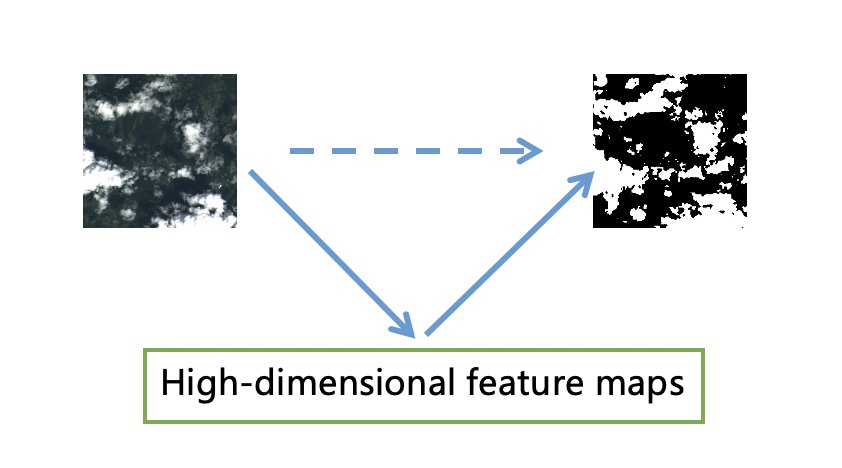
\includegraphics[scale=0.3]{../pic/en-decoder.jpg}
    \caption{encoder-decoder框架}
    \label{fig:en-decoder}
\end{figure}


目前也有很多方法将全卷积网络应用于遥感图像的云检测。Jeppesena等人\cite{jeppesen2019cloud}将UNet应用于landsat遥感图像云检测。Chai等人\cite{chai2019cloud}将SegNet应用于landsat图像。hughes等人\cite{hughes2019high}将FCN应用于云检测。这些方法都是将光谱与空间特征进行混合提起,很少有人会针对遥感图像多波段的特点对神经网络的结构进行针对性的设计。

卷积神经网络确实可以有效提取图像空间信息,所以应用神经网络做遥感图像的云检测可以表现出较好的性能。但这些方法存在两个缺点:1. 需要大量的参数与昂贵的计算,如UNet有28million个参数。 2.这些模型的检测结果往往过于平滑,因为他们混合提取光谱特征与空间特征,我们称之为one-stage方法,他们从图像的输入就开始混合像元进行计算,这使得输出的掩膜很难再对单个像素提纯以至于结果非常平滑。

在这篇文章中,我们提出了一个新颖的、简单的、有效的网络,主要包括两个阶段。我们的模型简略图\ref{fig:spoon_simple}所示。
第一部分,光谱特征提取部分。特征是分类成功的关键,而光谱特征是遥感图像中最本质的特征。在这一部分,我们完全使用1*1的卷积核,不考虑空间信息,对图像进行光谱特征提取。好的光谱特征可以减轻模型的学习压力,使得后续的空间特征更加容易被提取。并且,我们将光谱特征提取的结果直达最后的分类层,使得云检测结果更加细腻。
第二部分,空间特征提取部分。这一部分,我们采用目前主流的空间特征提取框架--encoder-decoder框架。不同的是,经过第一部分我们已经得到了光谱特征,在这一步,我们不会再进行光谱维度的特征提取,而是对第一部分得到的每一个特征图作为一组,对每一组进行单独的卷积(Group Conv)。由于第部分的存在,GC使我们的空间特征提取部分变得廉价且有效。
实验结果表明,该方法可以在模型参数大大减小的情况下,明显提高云检测精度。

\begin{figure}[H]
    \centering
    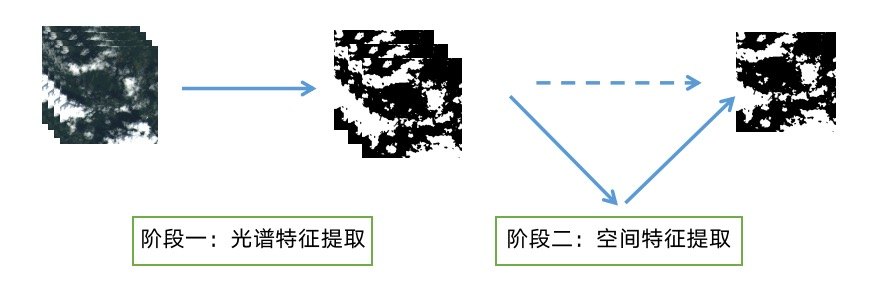
\includegraphics[scale=0.26]{../pic/spoon_simple.jpg}
    \caption{our net architecture.}
    \label{fig:spoon_simple}
\end{figure}

\section[]{Materials and Methods}
\subsection{Training and Evaluation Data}
我们采用的光学遥感卫星数据集来自NASA landsat8卫星。2013年2月11日,美国航空航天局(NASA) 成功发射Landsat-8卫星。Landsat-8卫星上携带两个传感器,分别是OLI陆地成像仪(Operational Land Imager)和TIRS热红外传感器(Thermal Infrared Sensor)。OLI提供9个波段,波段范围从0.43um到2.30um;TIRS提供地表温度数据,包括两个波段,波段范围从10.60um到12.51um,具体信息见表\ref{landsatBand}。landsat系列卫星每16天可以实现一次全球覆盖。
\begin{table}[H]
    \centering
    \begin{tabular}{c|c|c|c}
    \hline
    \hline
    传感器类型& 波段 &波长范围($\mu m$)& 空间分辨率\\
    \hline
    \multirow{9}*{OLI}& 1.Coastal& 0.433-0.453& 30\\
    ~&2.Blue& 0.450-0.515& 30\\
    ~&3.Green& 0.525-0.600& 30\\
    ~&4.Red& 0.630-0.680& 30\\
    ~&5.NIR& 0.845-0.885& 30\\
    ~&6.SWIR1& 1.56-1.66& 30\\
    ~&7.SWIR2& 2.1-2.3& 30\\
    ~&8.Pan& 0.5-0.68& 15\\
    ~&9.Cirrus& 1.36-1.39& 30\\
    \hline
    \multirow{2}*{OLI}& 10.TIRS1& 10.60-11.19& 100\\
    ~& 11.TIRS2& 11.50-12.51& 100\\
    \hline
    \hline
    \end{tabular}
    \caption{landsat8波段信息}
    \label{landsatBand}
    \end{table}


为了对模型进行训练与测试,我们利用已有的全球云和云影验证数据集
“L8 Biome Cloud Validation Masks”\cite{foga2017cloud_data},该数据集共有96景图片,包含8个种类的下垫面(including Barren, 
Forest,Grass/Crops, Shrubland, Snow/Ice, Urban, Water, Wetlands。

\begin{figure}[H]
    \centering
    \includegraphics[scale=0.5]{../pic/BiomeData.png}
    \caption{Global distribution of the 96 unique Landsat 8 Cloud Cover Assessment (CCA) scenes.}
    \label{fig:label}
\end{figure}

每景图片的标签均是人工标注,可信度较高。每个文件包含.TIF格式的Landsat 8 Level-1数据文件、质量文件和.img(ENVI)格式的真值标签,人工标志位如表\ref{BiomeFlag}所示。

\begin{table}[H]
    \centering
    \begin{tabular}{c|ccccc}
    \hline
    \hline
    value& 0& 64& 128& 192& 255\\
    \hline
    Interpretation&	Fill& Cloud Shadow& Clear &Thin Cloud& Cloud\\
    \hline
    \hline
    \end{tabular}
    \caption{L8 Biome 数据人工标注标志位}
    \label{BiomeFlag}
    \end{table}

根据云量百分比的多少,‘L8 Biome’中96景分为clear, midcloud, cloud三种,每种各占三分之一,云量低于35\%的为clear,云量高于65\%的为cloud,云量介于35\%与65\%之间的为midcloud。本文使用midcloud的所有数据,共32景做实验,每种地物有4景。数据我们将标签简单地分为云与非云两类,将每景L8图像均匀切割为256*256大小的小图,切割时过滤掉带填充值的图片,因此,图像边缘的填充像素并不会出现在训练与测试的步骤中。波段选择了除了全色波段的所有波段,共10个波段,训练集与测试集的比例为6:4,训练集有10247张子图,测试集有6932张子图。

\subsection{Network Architechture}

我们的模型是一个两阶段模型,第一阶段是光谱特征提取阶段,第二阶段是空间特征提取阶段,模型结构如图\ref{fig_myModel}所示。
\begin{figure}[H]
    \centering
    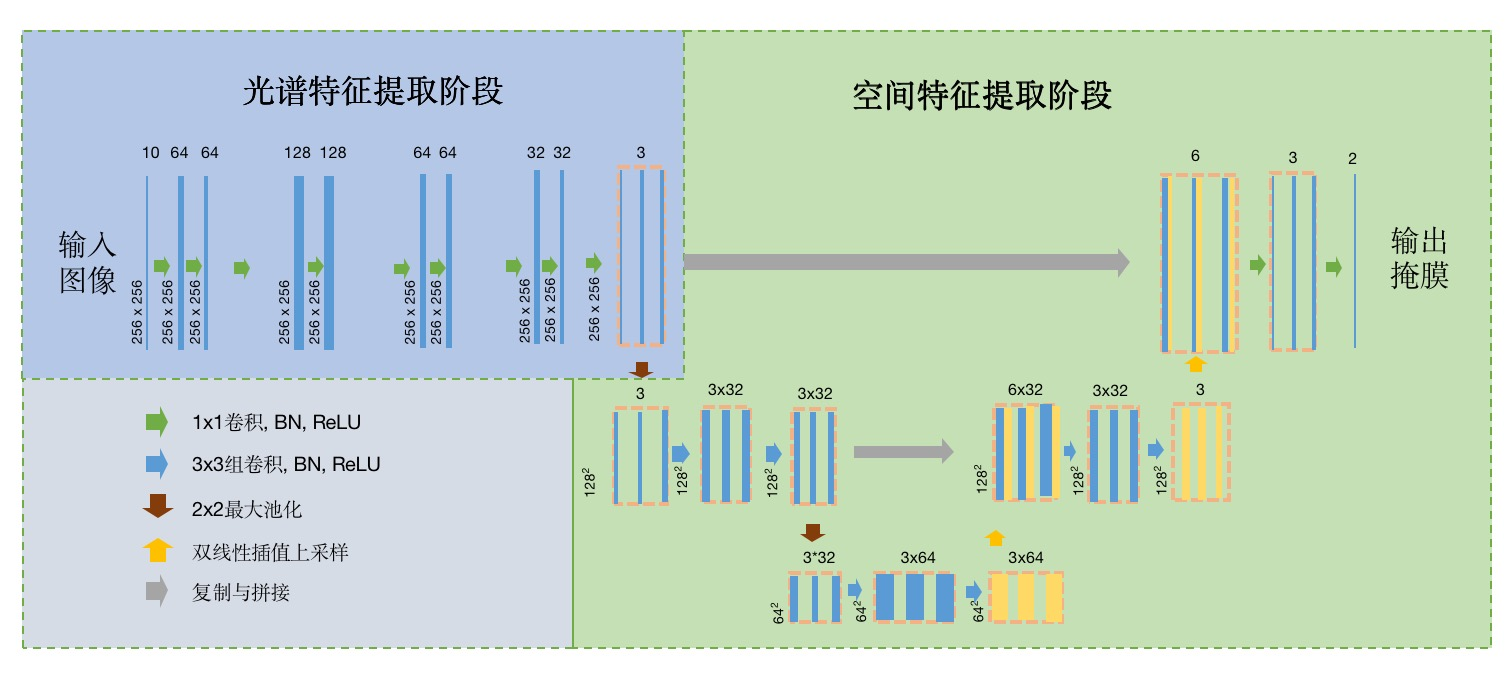
\includegraphics[scale=0.26]{../pic/spoon.jpg}
    \caption{our net architecture.}
    \label{fig_myModel}
\end{figure}

1. 光谱特征提取阶段。 该阶段等价于一个多层感知机(MLP),多层的神经网络可以有效提取非线性光谱特征,为后续分类提供良好的特征,并且不会降低图像分辨率,使用1*1的卷积核在图像上对每个像素卷积实现。这一阶段输出的每一个通道都是一种有效的光谱特征,类似于NDVI、NDWI之类,但远比它们复杂得多,也更有有效。这一阶段输出3个通道,我们认为3个通道是足够的因为人眼可以在彩色图像上很好的识别云。

\begin{figure}[H]
    \centering
    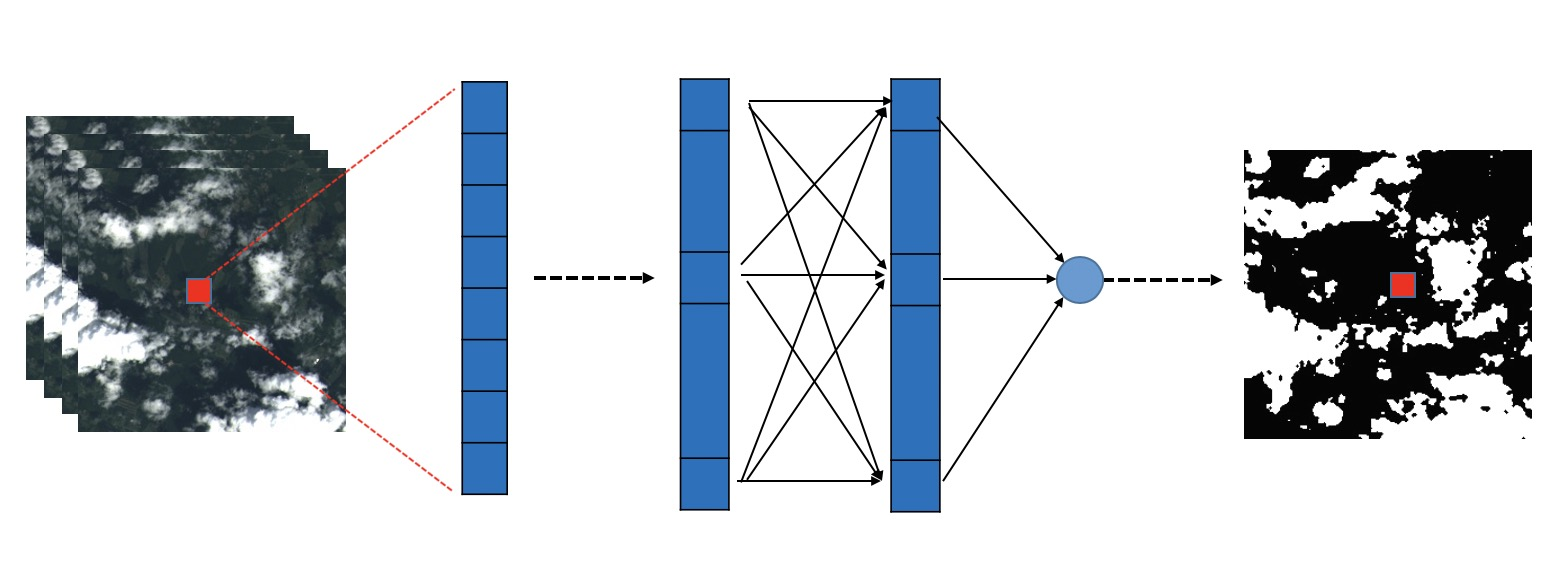
\includegraphics[scale=0.25]{../pic/part1.jpg}
    \caption[]{Part1. Straight access, 所有的卷积核都是1*1大小的,等价于多层感知机。}
    \label{pic:straight}
\end{figure}

若是不考虑图像的空间信息,对于遥感图像,我们使用决策树或者SVM也是可以对遥感图像的单个像素进行分类的,方法就是将每个像素单独地看作一个样本。事实上,很多方法就是这样做的,如zhu等人提出的FMask\cite{zhu2012object}。

2. 空间信息提取阶段。光谱特征虽然可以保持分辨率、解析细节,但它们不包含特定于区域的信息与上下文信息,容易造成较高的虚警率,因此我们仍需要提取空间信息去优化。图\ref{pic:part2}展示了每一组光谱特征的卷积过程。

\begin{figure}[H]
    \centering
    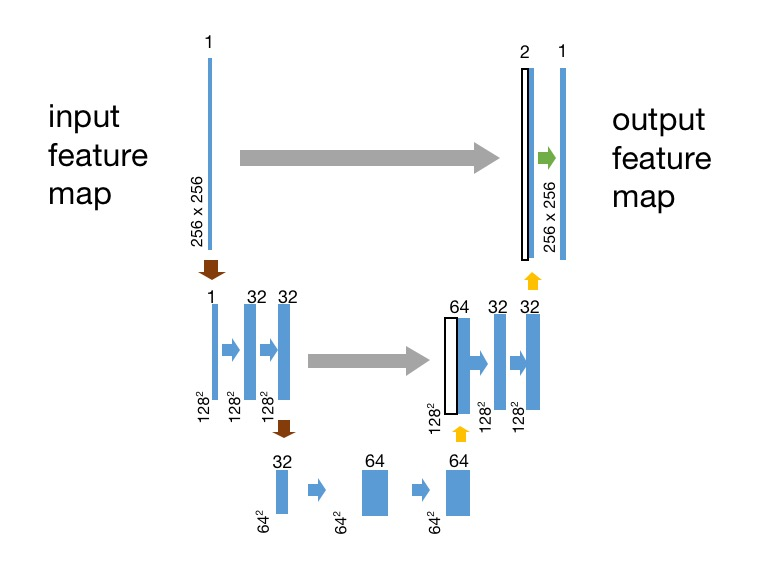
\includegraphics[scale=0.3]{../pic/groupcov.jpg}
    \caption[]{Part2. 每组特征图的卷积过程。}
    \label{pic:part2}
\end{figure}

为降低模型复杂度,减少模型过拟合的几率,做了两方面改进。第一,减少encoder-decoder层数。由于光谱特征提取部分的存在,在这一部分模型提取空间信息的压力已经被大大减小,所以我们并不需要很深的网络、很多的参数去拟合很复杂的空间特征,因此我们可以大胆减少encoder-decoder层数,而随着层数的减少,参数量几乎是几何减少的。第二,我们引入组卷积的概念。通过第一部分我们已经得到非常有效的光谱特征,我们在这一部分不会再重复地计算光谱特征,因此我们对每一层由同一光谱特征提取出来的空间特征进行分组,在每个小组内进行单独的卷积。图\ref{pic:GC}展示了组卷积与普通卷积的区别。

\begin{figure}[H]
    \centering
    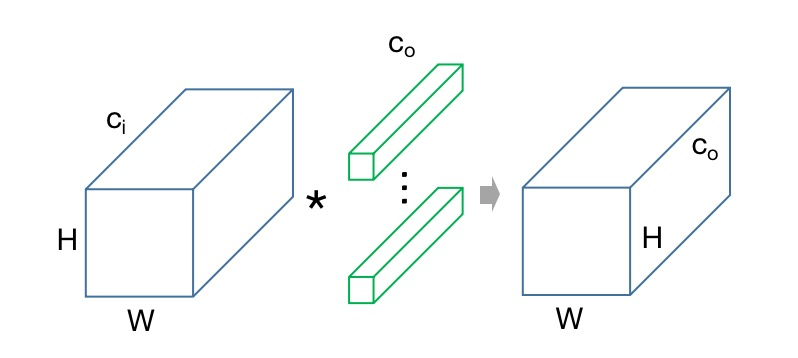
\includegraphics[scale=0.3]{../pic/conv.jpg}
    \caption[]{组卷积与普通卷积的区别。}
    \label{pic:GC}
\end{figure}

% 同时,为了以较小的代价捕获多尺度信息,借鉴deeplab的思想\cite{chen2017deeplab},引入金字塔型空洞卷积。由池化层获得的感受野信息会造成精度的损失,空洞卷积可以在不增加额外参数与下采样层的前提下提高感受野。
% 空洞卷积实际卷积核大小:$K=k+(k-1)(r-1)$,$k$为原始卷积核大小,$r$为空洞卷积参数空洞率。空洞率为1的空洞卷积就是正常的卷积。空洞卷积可以分为串联与并联两种情况,串联的情况比较复杂,我们选择了较为简单的并联结构。

% \begin{figure}[H]
%     \centering
%     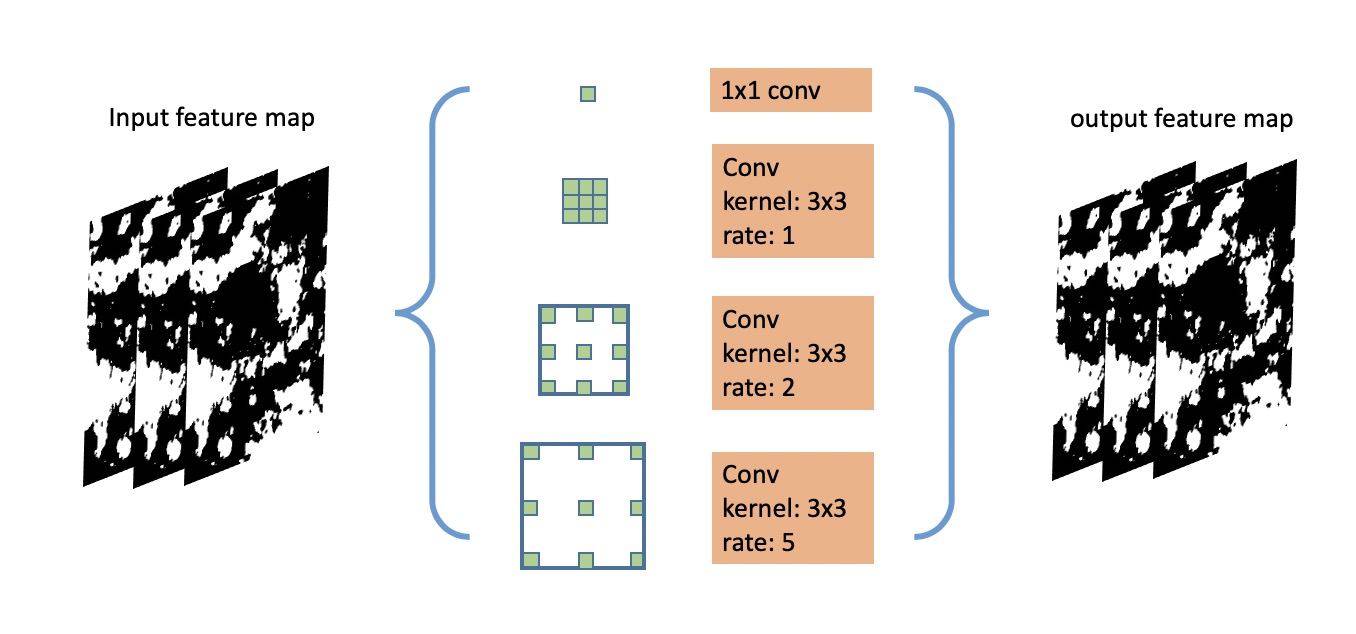
\includegraphics[scale=0.25]{../pic/aspp.jpg}
%     \caption[]{金字塔形空洞卷积(ASPP). 利用不同空洞率的卷积核收集不同尺度的信息。}
%     \label{pic:aspp}
% \end{figure}

% 3. 加入注意门控(Attention Gate)。我们利用attention gate将光谱信息与空间信息更加有效地融合起来。近年来,有很多研究将attention机制加入到语义分割模型中来。在神经网络中,非线性主要来源于激活函数与池化,attention的引入增加了非线性,一部分人以此来解释attention的有效性。为了获得足够大的感受野,feature map在CNN中被逐渐下采样。这样,特征与像素间的相对关系可以在一个大的视野中被收集。但是,这对于一些小但具有明显特征的目标并不友好。
% 目前大多数网络会在感受野最大的卷积位置增加attention结构,以此来学习全局的有效信息。我们考虑到,在云检测任务中应该更加注重下垫面与局部信息,因此,我们只在decoder的最后一层加入了attention机制。并且,这不会增加大量的额外参数。
% 令直达网络的输出为特征$f$,decoder的输出为门控信号$g$,那么我们的AG参考了\cite{oktay2018attention}中的结构,可以表示为图\ref{pic:AG}。

% \begin{figure}[H]
%     \centering
%     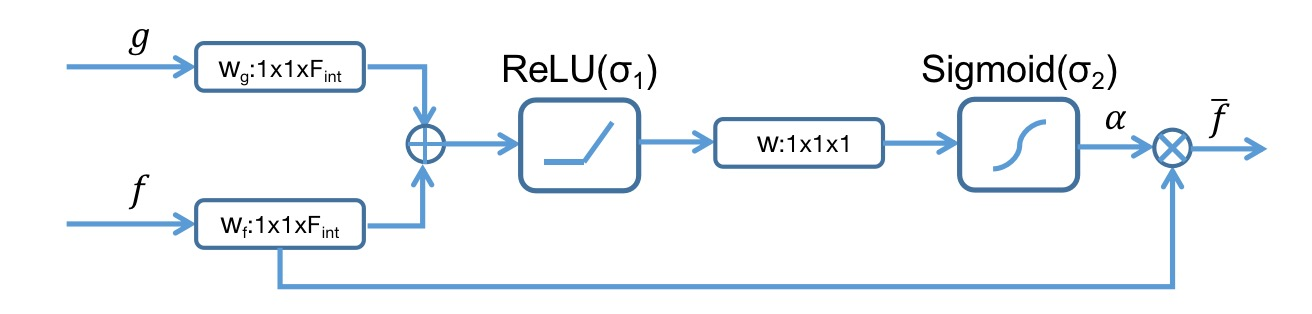
\includegraphics[scale=0.25]{../pic/AG.jpg}
%     \caption[]{Part3. Attention gate}
%     \label{pic:AG}
% \end{figure}

% 门控系数$\alpha$是长宽与输入特征$f$相同,但通道数为1的单层权重图,$\alpha_i\in[0,1]$。$w:1*1*1$意思是$w:height,weight,out\_channelss$。$w_g$与$w_f$将门控信号$g$和输入特征$f$变为形状完全相同的两个张量,$w$将输入张量变为2维的平面图,最后再由$Sigmoid$函数将实域映射到0-1之间。注意力机制的公式表述如下,其中$\sigma_1(x)=max(0,x)$,$\sigma_2(x)=\frac{1}{1+e^{-x}}$。
% \begin{equation}
%     \beta = \sigma_1(W_g^Tg+W_f^Tf+b_1)
% \end{equation}
% \begin{equation}
%     \alpha = \sigma_2(W^T\beta+b_2)
% \end{equation}

上采样的方式一般有四种:插值法,反卷积,反池化,超分辨率重建领域的亚像素卷积插值。双线性插值是目前在语义分割中用的比较多的一种插值方式,比如FCN中就是用的这种方法。在CNN上下文中,反卷积是卷积的逆过程,卷积用于提取空间信息,反卷积用于解析空间信息。在实现上,反卷积是卷积的转置,所以反卷积也叫做转置卷积。反池化是池化的逆过程,在池化过程中,记录下max-pooling在对应kernel中的坐标,在反池化过程中,将一个元素根据kernel进行放大,根据之前的坐标将元素填写进去,其他位置补0 。在下采样的时候记录max的位置,上采样的时候最大值的位置还原,其它位置填0。反池化是速度最快的上采样操作,计算量和参数也特别少,但是准确率一般。虽然理论上,由于反卷积具有更多的参数,所以反卷积可以更好的学习特征,但是有研究表明,如果参数配置不当,反卷积很容易出现输出feature map带有明显棋盘状的现象\cite{odena2016deconvolution},双线性差值可以取得与反卷积相同甚至更好的效果。因此,我们选择参数少且容易取得较好效果的双线性差值法。


在卷积之后,激活函数之前,一般会有一个批归一化操作\cite{ioffe2015batch}(Batch Normalization)。BN是一种非常优雅的重参数化的方法,它的存在类似于为网络中不同的层设置了不同的学习率。为神经网络输入的多个数据称为batch,BN以batch为单位,先将上一层网络的输出在通道上标准化为标准正态分布,再进行缩放与平移操作,可以将上一层的输出调整在一个较好的范围内,结果就是模型训练更加容易。

\begin{equation}
    BN(x) = \gamma\frac{x-\mu}{\sigma}+\beta
\end{equation}

本文中几乎所有的激活函数都是ReLU函数,$\sigma(x)=max(0,x)$。ReLU函数是一种分段线性函数,把所有的负值都变为0,而正值不变,这种操作被成为单侧抑制。单侧抑制使得神经网络中的神经元也具有了稀疏激活性。我们认为对于某种地物可以对某个特殊的指标有响应,而对其他指标就反应一般。所以ReLU实现稀疏后的模型能够更好地挖掘相关特征,且ReLU由于非负区间的梯度为常数,因此不存在梯度消失问题,使得模型的收敛速度维持在一个稳定状态。

\begin{equation}
    ReLU(x)=\left\{
    \begin{aligned}
        x, & &\text{if} & & x > 0 \\
        0, & &\text{if} & & x \leq 0
    \end{aligned}
    \right.
\end{equation}

在最后一层卷积层,激活函数会使用sigmoid函数,用于将输出映射到0-1之间,代表该像素点为云的概率。为了训练模型,使用交叉熵损失函数计算损失,并用带动量的随即梯度下降法进行训练。
\begin{equation}
    L = -\sum_{i=1}^N y_ilog(\hat{y}_i)+(1-y_i)log(1-\hat{y}_i)
\end{equation}
其中,$N$表示所有所有样本个数,$y_i$代表标签真值,$\hat{y_i}$代表模型预测值。

\section[]{Experience and Result}

为客观评定算法的有效性和优越性,采用准确率,召回率,精确度,$F_1$值对结果进行评估。其中,准确率衡量像素分类正确的概率;召回率衡量属于云的像素中被分类正确的概率,是漏警率的相反数;精确度衡量被识别为云的像素中真正是云的概率,是虚警率的相反数;$F_1$值是召回率与精确度的调和平均数,常被用于二分类问题,可以有效衡量样本不均衡时检测结果的好坏。四个评价指标分别为:

\begin{equation}
    A = \frac{TP + TN}{TP + TN + FP + FN}\label{acc}
\end{equation}
\begin{equation}
    R = \frac{TP}{TP + FN}\label{recall}
\end{equation}
\begin{equation}
    P = \frac{TP}{TP + FP}\label{precision}
\end{equation}
\begin{equation}
    F = \frac{2 * R_{recall} * R_{precision}}{R_{recall} + R_{precision}}\label{f1}
\end{equation}

其中,TP为真正类(True Positive),即云被判为云;TN为真负类(True Negative),即非云被判为非云;FP为假正类(False Positive),即非云被判为云;FN为假负类(false Negative),云被判为非云。

本文将模型与CFMask、原始的UNet做比较。输入是除了全色波段的其余10个波段,将所有图像按6:4随机划分为训练集和测试集,并调整UNet的输入通道数为10。将ground truth分为云与非云两类。有研究表明\cite{chai2019cloud}输入DN或TOA数据,会取得相似的结果,我们选择使用DN值作为模型输入,并为了使训练更加稳定,对输入进行归一化。
具体参数,如学习率为$1e^{-2}$,batch size 为 8,采用动量为0.9的随即梯度下降法训练。我们的损失函数包括两部分,分别计算光谱与空间特征提取两阶段的损失\ref{pic:loss}。为了使模型更加容易收敛,auxiliary loss的权重逐渐降低,final loss的权重逐渐增高,分为3个阶段:(0.8, 0.2)、(0.2, 0.8)、(0, 1)。

\begin{figure}[H]
    \centering
    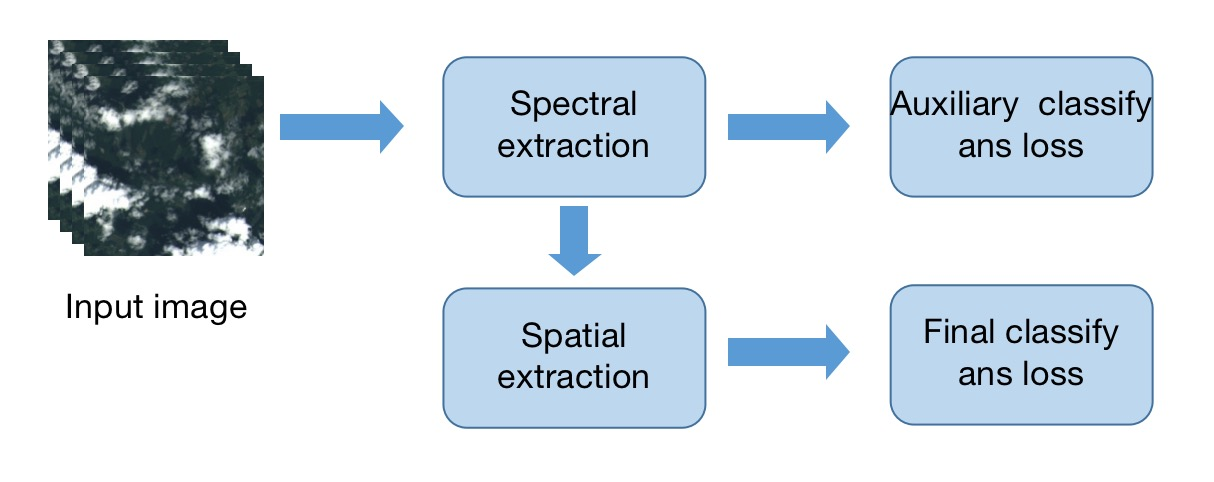
\includegraphics[scale=0.25]{../pic/loss.jpg}
    \caption[]{损失函数采用交叉熵损失,除了最终的分类损失,在光谱特征提取部分增加了辅助损失。}
    \label{pic:loss}
\end{figure}

如表(\ref{tab_eval})所示,相比于CFMask,取得了8个百分点的性能提升;在模型参数量只有unet的八十分之一的情况下,准确率和f1值均高于unet,更加轻量,具有更大的应用潜力。所有实验均在MacBook Pro (15-inch, 2018)上进行,处理器为2.2 GHz Intel Core i7,内存16 GB 2400 MHz DDR4,Intel UHD Graphics 630 1536 MB。

\begin{table}[H]
    \centering
    \resizebox{\textwidth}{!}{
    \begin{tabular}{c|cccccccccc}
        \hline
        \hline
        model& evaluation& Barren& Forest& Grass/Crops& Shrubland& Snow/Ice& Urban& Water&  Wetlands& total\\
        \hline
        \multirow{4}*{SpoonNet}
        % &acc   &94.74 &96.22 &94.31 &94.08 &94.62 &94.22 &94.63 &92.84 &\textbf{94.46}\\
        % &rec.  &97.83 &95.92 &91.36 &93.66 &96.39 &97.83 &93.80 &99.16 &\textbf{95.75}\\
        % &prec. &93.88 &98.70 &92.72 &95.00 &91.18 &89.78 &92.62 &89.35 &92.90\\
        % &F1    &95.82 &97.29 &92.04 &94.33 &93.71 &93.63 &93.21 &94.00 &\textbf{94.25}\\
        &acc   &96.16 &95.46 &93.08 &94.91 &94.52 &95.11 &94.21 &94.11 &\textbf{94.69}\\
        &rec.  &95.69 &94.20 &83.34 &92.55 &90.03 &95.49 &90.55 &98.26 &\textbf{92.51}\\
        &prec. &98.01 &99.35 &97.02 &97.63 &96.58 &93.39 &94.49 &91.88 &\textbf{96.05}\\
        &F1    &96.84 &96.71 &89.66 &95.02 &93.19 &94.43 &92.48 &94.97 &\textbf{94.16}\\
        \hline
        \multirow{4}*{U-Net}
        &acc   &96.09 &94.51 &92.67 &94.48 &91.78 &95.00 &93.74 &94.90 &94.15\\
        &rec.  &96.00 &92.96 &81.91 &91.58 &89.16 &96.22 &89.83 &98.34 &92.00\\
        &prec. &97.60 &99.22 &97.31 &97.77 &90.90 &92.56 &93.97 &93.05 &95.30\\
        &F1    &96.80 &95.99 &88.95 &94.58 &90.02 &94.36 &91.85 &95.62 &93.52\\
        \hline
        \multirow{4}*{CFMask}
        &acc   &87.46 &95.20 &85.42 &90.34 &60.97 &83.05 &91.51 &90.78 &86.09\\
        &rec.  &90.85 &93.87 &68.03 &92.04 &92.21 &96.07 &92.22 &96.37 &91.45\\
        &prec. &88.99 &99.31 &88.85 &89.83 &51.74 &73.25 &86.97 &88.38 &82.89\\
        &F1    &89.91 &96.51 &77.05 &90.92 &66.29 &83.13 &89.52 &92.21 &86.96\\
        \hline
        \hline
    \end{tabular}}
    \caption{Evaluation results on the Biome dataset}
    \label{tab_eval}
\end{table}

在大部分情况下,我们的模型与U-Net相差无几。但可以发现,我们的模型对于碎云、细节有良好的检测与保持能力。unet的识别更加光滑,使得一些细节被忽略,而我们的模型更加注重细节,这对于云检测是一个很重要的能力。如图\ref{Fig.main1}所示,从左到右依次为真彩色图、人工标注、光谱特征提取结果、我们的模型预测结果、UNet结果,白色代表云,黑色代表非云,第二行是第一行黄色方框的放大图,以此类推。我们的模型由于有光谱特征提取层的存在,并且光谱特征直达最后的分类层,所以对细节有较好的保持,对碎云有良好的识别,能以极少的参数在整体上达到与U-Net相近的效果。

\begin{figure}[H]
    \centering
    \subfigure[Color]{
        \begin{minipage}[b]{0.15\linewidth}
            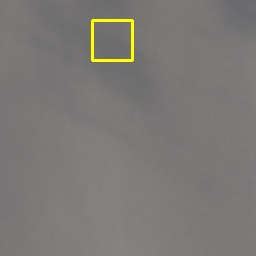
\includegraphics[width=1\linewidth]{../log/spoon2/cut/LC81321192014054LGN00_03055_color.jpg}\vspace{4pt}
            
\includegraphics[width=1\linewidth]{../log/spoon2/cut/tmp_cut_LC81321192014054LGN00_03055_color.jpg}\vspace{4pt}
            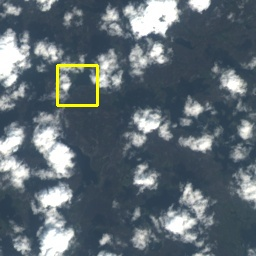
\includegraphics[width=1\linewidth]{../log/spoon2/cut/LC80350192014190LGN00_06561_color.jpg}\vspace{4pt}
            
\includegraphics[width=1\linewidth]{../log/spoon2/cut/tmp_cut_LC80350192014190LGN00_06561_color.jpg}\vspace{4pt}
            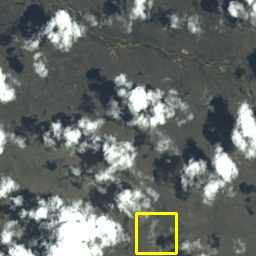
\includegraphics[width=1\linewidth]{../log/spoon2/cut/LC80980712014024LGN00_15443_color.jpg}\vspace{4pt}
            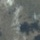
\includegraphics[width=1\linewidth]{../log/spoon2/cut/tmp_cut_LC80980712014024LGN00_15443_color.jpg}\vspace{4pt}
        \end{minipage}
    }
    \subfigure[GT]{
        \begin{minipage}[b]{0.15\linewidth}
            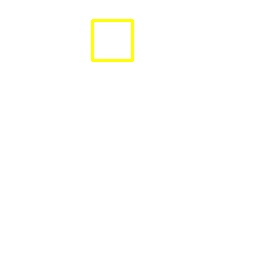
\includegraphics[width=1\linewidth]{../log/spoon2/cut/LC81321192014054LGN00_03055_mask.jpg}\vspace{4pt}
            
\includegraphics[width=1\linewidth]{../log/spoon2/cut/tmp_cut_LC81321192014054LGN00_03055_mask.jpg}\vspace{4pt}
            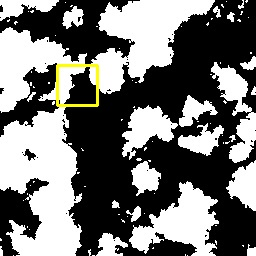
\includegraphics[width=1\linewidth]{../log/spoon2/cut/LC80350192014190LGN00_06561_mask.jpg}\vspace{4pt}
            
\includegraphics[width=1\linewidth]{../log/spoon2/cut/tmp_cut_LC80350192014190LGN00_06561_mask.jpg}\vspace{4pt}
            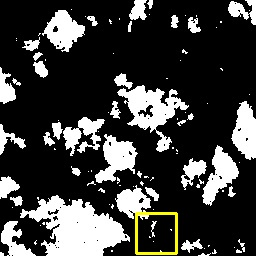
\includegraphics[width=1\linewidth]{../log/spoon2/cut/LC80980712014024LGN00_15443_mask.jpg}\vspace{4pt}
            
\includegraphics[width=1\linewidth]{../log/spoon2/cut/tmp_cut_LC80980712014024LGN00_15443_mask.jpg}\vspace{4pt}
        \end{minipage}
    }
    \subfigure[Spectral]{
        \begin{minipage}[b]{0.15\linewidth}
            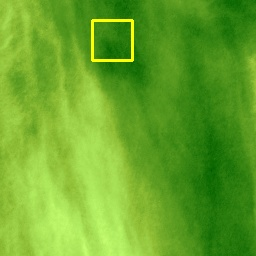
\includegraphics[width=1\linewidth]{../log/spoon2/cut/LC81321192014054LGN00_03055_spectral.jpg}\vspace{4pt}
            
\includegraphics[width=1\linewidth]{../log/spoon2/cut/tmp_cut_LC81321192014054LGN00_03055_spectral.jpg}\vspace{4pt}
            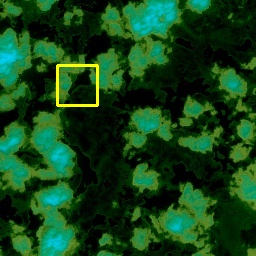
\includegraphics[width=1\linewidth]{../log/spoon2/cut/LC80350192014190LGN00_06561_spectral.jpg}\vspace{4pt}
            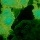
\includegraphics[width=1\linewidth]{../log/spoon2/cut/tmp_cut_LC80350192014190LGN00_06561_spectral.jpg}\vspace{4pt}
            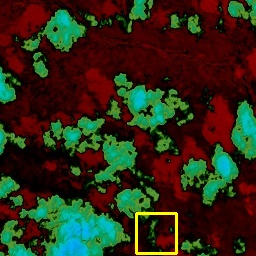
\includegraphics[width=1\linewidth]{../log/spoon2/cut/LC80980712014024LGN00_15443_spectral.jpg}\vspace{4pt}
            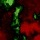
\includegraphics[width=1\linewidth]{../log/spoon2/cut/tmp_cut_LC80980712014024LGN00_15443_spectral.jpg}\vspace{4pt}
        \end{minipage}
    }
    \subfigure[SNet]{
        \begin{minipage}[b]{0.15\linewidth}
            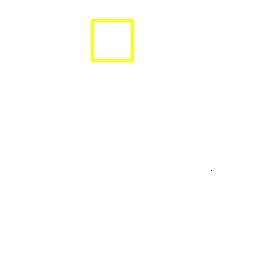
\includegraphics[width=1\linewidth]{../log/spoon2/cut/LC81321192014054LGN00_03055_my.jpg}\vspace{4pt}
            
\includegraphics[width=1\linewidth]{../log/spoon2/cut/tmp_cut_LC81321192014054LGN00_03055_my.jpg}\vspace{4pt}
            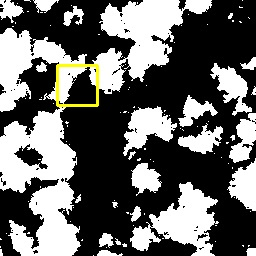
\includegraphics[width=1\linewidth]{../log/spoon2/cut/LC80350192014190LGN00_06561_my.jpg}\vspace{4pt}
            
\includegraphics[width=1\linewidth]{../log/spoon2/cut/tmp_cut_LC80350192014190LGN00_06561_my.jpg}\vspace{4pt}
            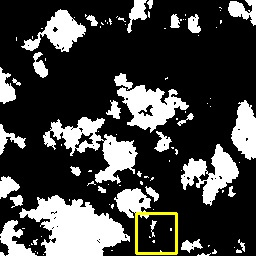
\includegraphics[width=1\linewidth]{../log/spoon2/cut/LC80980712014024LGN00_15443_my.jpg}\vspace{4pt}
            
\includegraphics[width=1\linewidth]{../log/spoon2/cut/tmp_cut_LC80980712014024LGN00_15443_my.jpg}\vspace{4pt}
        \end{minipage}
    }
    \subfigure[UNet]{
        \begin{minipage}[b]{0.15\linewidth}
            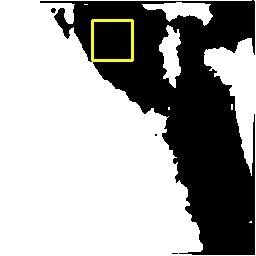
\includegraphics[width=1\linewidth]{../log/spoon2/cut/LC81321192014054LGN00_03055_unet.jpg}\vspace{4pt}
            
\includegraphics[width=1\linewidth]{../log/spoon2/cut/tmp_cut_LC81321192014054LGN00_03055_unet.jpg}\vspace{4pt}
            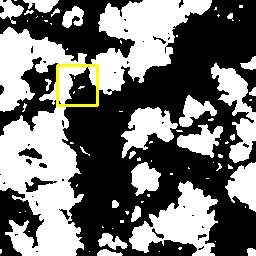
\includegraphics[width=1\linewidth]{../log/spoon2/cut/LC80350192014190LGN00_06561_unet.jpg}\vspace{4pt}
            
\includegraphics[width=1\linewidth]{../log/spoon2/cut/tmp_cut_LC80350192014190LGN00_06561_unet.jpg}\vspace{4pt}
            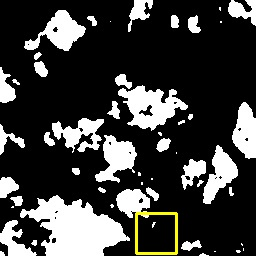
\includegraphics[width=1\linewidth]{../log/spoon2/cut/LC80980712014024LGN00_15443_unet.jpg}\vspace{4pt}
            
\includegraphics[width=1\linewidth]{../log/spoon2/cut/tmp_cut_LC80980712014024LGN00_15443_unet.jpg}\vspace{4pt}
        \end{minipage}
    }
\caption{Example of prediction,(a)(b)(c)(d)(e)分别为真彩色图、真实地物、第一部分提取的光谱特征、SNet
的预测结果、UNet的预测结果,白色代表云,黑色代表非云}
\label{Fig.main1}
\end{figure}

我们的模型参数量有0.35M,而主流网络如U-Net有28M,FCN有20.5M。其他网络参数多的主要原因是具有更深的encoder-decoder结构,以U-Net为例,U-Net最深一层就有14M的参数,占据了所有参数的一半。
我们的模型由于更加注重单个像素的光谱特征,在提取空间信息之前先使用少量的参数(1*1卷积核)提取光谱信息,使得我们可以大胆的减少encoder-decoder层数,同时引入组卷积的操作,极大地简化模型,大大降低参数量。

% \begin{table}[H]
%     \centering
%     \resizebox{\textwidth}{!}{
%     \begin{tabular}{c|cccccccccc}
%         \hline
%         \hline
%         model& evaluation& Barren& Forest& Grass/Crops& Shrubland& Snow/Ice& Urban& Water&  Wetlands& total\\
%         \hline
%         \multirow{4}*{S-Net}
%         &rec.  &5.54 &50.49 &25.13 &31.62 &6.21 &31.11 &28.15 &25.77 &25.50\\
%         &prec. &6.89 &50.10 &26.27 &32.82 &2.98 &18.65 &21.81 &30.42 &23.74\\
%         &F1    &6.14 &50.30 &25.69 &32.21 &4.03 &23.32 &24.58 &27.90 &24.27\\
%         \hline
%         \multirow{4}*{U-Net}
%         &rec.  &14.23 &20.88 &25.69 &23.24 &6.02 &27.66 &16.72 &27.10 &20.19\\
%         &prec. &24.52 &29.39 &37.55 &32.66 &3.33 &27.08 &19.52 &42.50 &27.07\\
%         &F1    &18.01 &24.42 &30.51 &27.16 &4.29 &27.37 &18.01 &33.10 &22.86\\
%         \hline
%         \multirow{4}*{CFMask}
%         &rec.  &8.80 &56.97 &23.26 &23.65 &4.33 &22.62 &28.21 &19.00 &23.36\\
%         &prec. &3.60 &47.16 &16.09 &12.41 &0.50 &12.81 &8.48 &12.58 &14.20\\
%         &F1    &5.11 &51.60 &19.02 &16.28 &0.89 &16.35 &13.04 &15.14 &17.18\\
%         \hline
%         \hline
%     \end{tabular}}
%     \caption{Evaluation results on the Biome dataset}
%     \label{tab_eval}
% \end{table}

而且,有研究表明\cite{scaramuzza2011development}人工标注的数据可能存在7\%左右的错误。尤其对于一些碎云、半透明的薄云,评判标准可能会因人而异。我们发现,'L8 Biome'数据确实存在一些问题。同时,由于人工标注的不稳定性,简单地依靠评价指标可能并不能真实反应模型的优劣,因为大部分模型都很容易对于大面积的厚云(低下垫面信息的)有较好的识别能力;并且以这些标签为真值进行的训练,可能也会存在问题。

\begin{figure}[H]
    \centering
    \subfigure[Color]{
        \begin{minipage}[b]{0.15\linewidth}
            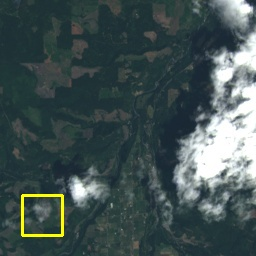
\includegraphics[width=1\linewidth]{../log/spoon2/cut2/LC80460282014171LGN00_12434_color.jpg}\vspace{4pt}
            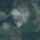
\includegraphics[width=1\linewidth]{../log/spoon2/cut2/tmp_cut_LC80460282014171LGN00_12434_color.jpg}\vspace{4pt}
            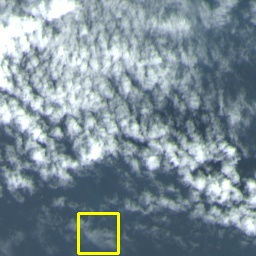
\includegraphics[width=1\linewidth]{../log/spoon2/cut2/LC81620432014072LGN00_16237_color.jpg}\vspace{4pt}
            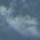
\includegraphics[width=1\linewidth]{../log/spoon2/cut2/tmp_cut_LC81620432014072LGN00_16237_color.jpg}\vspace{4pt}
            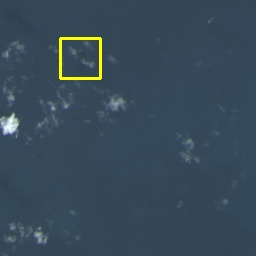
\includegraphics[width=1\linewidth]{../log/spoon2/cut2/LC81620432014072LGN00_16329_color.jpg}\vspace{4pt}
            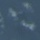
\includegraphics[width=1\linewidth]{../log/spoon2/cut2/tmp_cut_LC81620432014072LGN00_16329_color.jpg}\vspace{4pt}
        \end{minipage}
    }
    \subfigure[GT]{
        \begin{minipage}[b]{0.15\linewidth}
            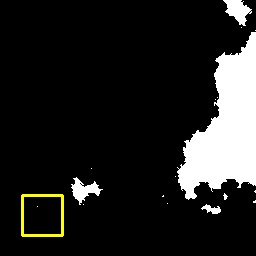
\includegraphics[width=1\linewidth]{../log/spoon2/cut2/LC80460282014171LGN00_12434_mask.jpg}\vspace{4pt}
            
\includegraphics[width=1\linewidth]{../log/spoon2/cut2/tmp_cut_LC80460282014171LGN00_12434_mask.jpg}\vspace{4pt}
            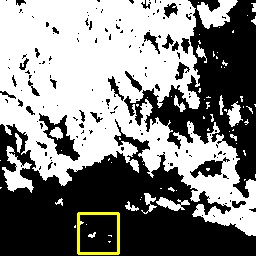
\includegraphics[width=1\linewidth]{../log/spoon2/cut2/LC81620432014072LGN00_16237_mask.jpg}\vspace{4pt}
            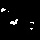
\includegraphics[width=1\linewidth]{../log/spoon2/cut2/tmp_cut_LC81620432014072LGN00_16237_mask.jpg}\vspace{4pt}
            \includegraphics[width=1\linewidth]{../log/spoon2/cut2/LC81620432014072LGN00_16329_mask.jpg}\vspace{4pt}
            \includegraphics[width=1\linewidth]{../log/spoon2/cut2/tmp_cut_LC81620432014072LGN00_16329_mask.jpg}\vspace{4pt}
        \end{minipage}
    }
    \subfigure[Spectral]{
        \begin{minipage}[b]{0.15\linewidth}
            \includegraphics[width=1\linewidth]{../log/spoon2/cut2/LC80460282014171LGN00_12434_spectral.jpg}\vspace{4pt}
            \includegraphics[width=1\linewidth]{../log/spoon2/cut2/tmp_cut_LC80460282014171LGN00_12434_spectral.jpg}\vspace{4pt}
            \includegraphics[width=1\linewidth]{../log/spoon2/cut2/LC81620432014072LGN00_16237_spectral.jpg}\vspace{4pt}
            \includegraphics[width=1\linewidth]{../log/spoon2/cut2/tmp_cut_LC81620432014072LGN00_16237_spectral.jpg}\vspace{4pt}
            \includegraphics[width=1\linewidth]{../log/spoon2/cut2/LC81620432014072LGN00_16329_spectral.jpg}\vspace{4pt}
            \includegraphics[width=1\linewidth]{../log/spoon2/cut2/tmp_cut_LC81620432014072LGN00_16329_spectral.jpg}\vspace{4pt}
        \end{minipage}
    }
    \subfigure[SNet]{
        \begin{minipage}[b]{0.15\linewidth}
            \includegraphics[width=1\linewidth]{../log/spoon2/cut2/LC80460282014171LGN00_12434_my.jpg}\vspace{4pt}
            \includegraphics[width=1\linewidth]{../log/spoon2/cut2/tmp_cut_LC80460282014171LGN00_12434_my.jpg}\vspace{4pt}
            \includegraphics[width=1\linewidth]{../log/spoon2/cut2/LC81620432014072LGN00_16237_my.jpg}\vspace{4pt}
            \includegraphics[width=1\linewidth]{../log/spoon2/cut2/tmp_cut_LC81620432014072LGN00_16237_my.jpg}\vspace{4pt}
            \includegraphics[width=1\linewidth]{../log/spoon2/cut2/LC81620432014072LGN00_16329_my.jpg}\vspace{4pt}
            \includegraphics[width=1\linewidth]{../log/spoon2/cut2/tmp_cut_LC81620432014072LGN00_16329_my.jpg}\vspace{4pt}
        \end{minipage}
    }
    \subfigure[UNet]{
        \begin{minipage}[b]{0.15\linewidth}
            \includegraphics[width=1\linewidth]{../log/spoon2/cut2/LC80460282014171LGN00_12434_unet.jpg}\vspace{4pt}
            \includegraphics[width=1\linewidth]{../log/spoon2/cut2/tmp_cut_LC80460282014171LGN00_12434_unet.jpg}\vspace{4pt}
            \includegraphics[width=1\linewidth]{../log/spoon2/cut2/LC81620432014072LGN00_16237_unet.jpg}\vspace{4pt}
            \includegraphics[width=1\linewidth]{../log/spoon2/cut2/tmp_cut_LC81620432014072LGN00_16237_unet.jpg}\vspace{4pt}
            \includegraphics[width=1\linewidth]{../log/spoon2/cut2/LC81620432014072LGN00_16329_unet.jpg}\vspace{4pt}
            \includegraphics[width=1\linewidth]{../log/spoon2/cut2/tmp_cut_LC81620432014072LGN00_16329_unet.jpg}\vspace{4pt}
        \end{minipage}
    }
\caption{Example of bad GT。(a)(b)(c)(d)(e)分别为真彩色图、真实地物、第一部分提取的光谱特征、SNet
的预测结果、UNet的预测结果,白色代表云,黑色代表非云}
\label{Fig.main2}
\end{figure}

\section[]{Conclusion}
云检测一直是遥感领域的研究热点与难点。本文提出了一种两阶段的遥感图像云检测模型。相比于现有的深度学习模型,我们的模型更加轻量,并且具有更好的保持边缘细节的能力和对小的碎云的检测能力,这在云检测中非常重要。我们首先引入光谱特征提取部分,利用1*1的卷积核,使得检测结果保持了“纯粹性”,没有收到其空间信息的干扰,并使使其直达最终的分类层。再通过encoder-decoder结构,引入组卷积,对每个光谱特征分别计算空间信息。该模型充分利用遥感图像多波段的特点,在保持边缘细节与扩大感受野之间寻找矛盾的解决方法,并在landsat8数据集上达到了94.69\%的准确率,基本还原了输入影像的细节信息。后续将继续优化直达通道与空间信息提取部分,并尝试深度学习与传统方法结合,以实现更加精确的遥感图像云检测。

\bibliography{./ref.bib}
\end{document}
